%!TEX root = ../../main.tex

\newcommand{\importGQL}[2]{
    \lstinputlisting[
        caption={#2},
        label={ls:gql:#1}
    ]{src/code/#1.gql}   
}

\newcommand{\importHS}[2]{
    \lstinputlisting[
        language={haskell},
        caption={#2},
        label={ls:hs:#1}
    ]{src/code/#1.hs}   
}

\newcommand{\expr}[1]{\hspace{0.2mm}\mbox{\textcolor{green!35!blue!55!black}{\texttt{#1}}}}

\newcommand{\refGQL}[1]{Listing \ref{ls:gql:#1}}
\newcommand{\refHS}[1]{Listing \ref{ls:hs:#1}}

\section{Background}

\begin{frame}\frametitle{Haskell}

    \footnotesize
    \begin{block}{Haskell}
        Haskell is a non-strict, purely functional language with static typing and algebraic data types. It is a rich language that offers useful features such as currying, infix-prefix operations, anonymous functions, list comprehensions, and monads. In order to easily distinguish constructors, it allows only capitalized constructors and disallows them for variables. Besides, the language contains type system extensions like polymorphic recursion, higher-rank types, lexically scoped type variables, generic programming, template meta-programming,  and much more. Many developers think that Haskell programs look nice~\cite{history-of-haskell}.
    \end{block}

    \begin{block}{The following topics outline Haskell's main goals and principles}
    
        \begin{itemize}
            \item Haskell is lazy: 
            Laziness was indeed the primary concern in Haskell's design. Technically, Haskell is a non-strict semantic language; lazy evaluation is merely an implementation technique for a non-strict language.  However, since laziness has its price 
            , the language also offers some strict features~\cite{history-of-haskell}.
    
            \item Haskell is pure: Due to laziness, the evaluation sequence is demand-oriented, a function call can no longer guarantee reliable performance of side effects. Consequently, the pure design is inevitable. Since input and output operations can be painfully complicated without side effects, the Haskell developers have developed a new approach called monadic IO, which is one of Haskell's most important contributions to the world~\cite{history-of-haskell}.
        \end{itemize}

    \end{block}

\end{frame}

\begin{frame}\frametitle{Algebraic Data Types}

An algebraic data type is the sum of one or more alternatives, where each alternative is a product of zero or more fields (Haskell also allows a sum of zero alternatives, the so-called empty type)~\cite{history-of-haskell}. 

Algebraic data types and pattern matching are fundamental to most modern functional languages~\cite{trees-that-grow}. Using pattern matching against algebraic data types improves readability significantly~\cite{history-of-haskell}.
    

Listing  declares \expr{Maybe} as data type, with two data constructors, \expr{Nothing} and \expr{Just}. The values of type \expr{Maybe} take one of two forms: either \expr{Nothing} or \expr{Just x}. Constructors can be used in pattern matching to decompose both a value of type and an expression~\cite{history-of-haskell}. 
    
\importHS{maybe}{Algebraic Data Types~\cite{history-of-haskell}}

algebraic data types also have their limitations. Once a data type is defined and compiled, its definition cannot be extended by adding new data constructors (or new fields)~\cite{trees-that-grow}.

\end{frame}

\begin{frame}\frametitle{Records}
    
    Early versions of Haskell provided only positional notation and pattern matching to build and decompose user-defined data types. This positional notation is cumbersome and error-prone for handling data types with many components, which is quite common in real-world applications. Therefore, later versions of Haskell introduced minimalistic record syntax as a labeled field~\cite{lw-ext-records, history-of-haskell}.
The record system provides syntactic sugar for what might 
otherwise be written using ordinary, positional, 
algebraic data type declarations~\cite{lw-ext-records}. For example, 
the data type \expr{Deity} \seeHS{records-def} declares a regular algebraic data type, 
but at the same time, 
constructor field accessors and modifiers. 

\snippetHS{records}{Haskell Record}

Record characteristics bring significant advantages and greatly simplify programming with data structures that have many components. Since the individual components are accessed by name (not by position), the fields' ordering is not crucial~\cite{lw-ext-records}.
In \refHS{record-values}, for example, 
the same record value can be written either way.

However, records also introduce some considerable problems; for example, 
no field name can be used in more than one data type~\cite{lw-ext-records}.
Another weakness of Haskell record systems is that there is no support for extensibility. 
There are no operators for adding and removing fields in a record~\cite{poly-ext-records, hlist}. 
Moreover, labels are not first-class citizens, 
meaning we cannot reuse labels between different record types, 
nor can we treat labels as data~\cite{hlist}.
This missing feature gave rise to many discussions and proposals to support polymorphic extensible records with different approaches, such as \gls{trex} or \gls{h-list} \seeSection{hlist}~\cite{history-of-haskell, poly-ext-records, hlist, basic-tlp}.

\end{frame}


\begin{frame}{GraphQL}

    \footnotesize

    \begin{block}{Was ist GraphQL?}
        GraphQL ist eine API-Abfragesprache zur Lösung der Effizienzprobleme der Kommunikation\cite{gql-iot}.         
    \end{block}

    \begin{block}{von Facebook Entwicklt}
        Es wurde drei Jahre lang intern bei Facebook entwickelt und seine Spezifikation und seine Referenzimplementierung 2016 veröffentlicht.
        \cite{initial-analysis-of-gql}
    \end{block}

    \begin{block}{GraphQL als aktueller Trend}
        Seit ihrem ersten Erscheinen hat sie ein reiches Open-Source-Ökosystem und das Vertrauen von Unternehmen aus verschiedenen Sektoren gewonnen. z.B: (GitHub), Unterhaltung (Netflix), Finanzen (PayPal), Reisen (KLM), etc \cite{morph-gql-1,gql-healthcare}.
    \end{block}

\end{frame}






% \section{Morpheus GraphQL}
% \setBGColor{white}
% \begin{frame}{Morpheus GraphQL}
%     \begin{figure}
%         \centering
%         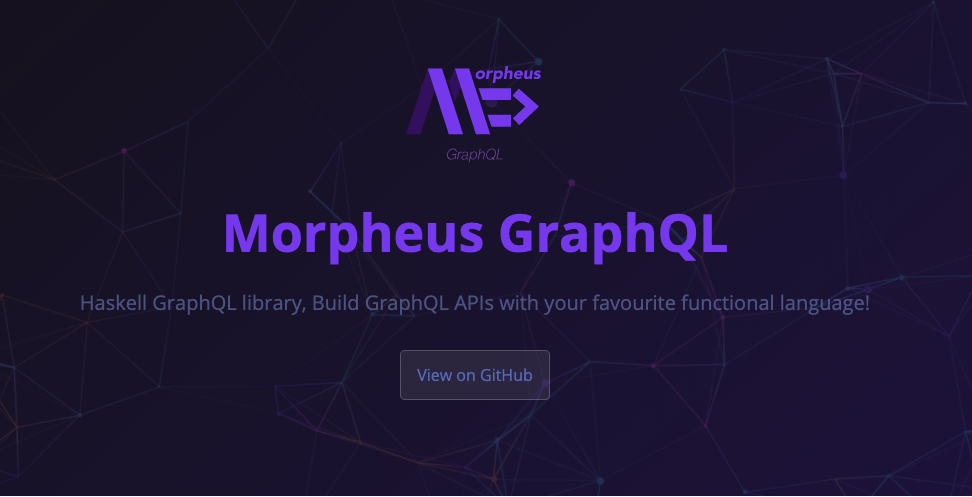
\includegraphics[width=1.1\textwidth]{assets/img/morpheus-graphql-bg.png}
%     \end{figure}
% \end{frame}